% =====================================================================
%  Frame "Edge TPU" : caracteristiques generales, image du Coral USB.
%  Remplace la frame a table de latences.
% =====================================================================
\begin{frame}
\frametitle{Edge TPU}

\vspace{0.35cm}

\begin{minipage}{0.42\textwidth}
\begin{center}
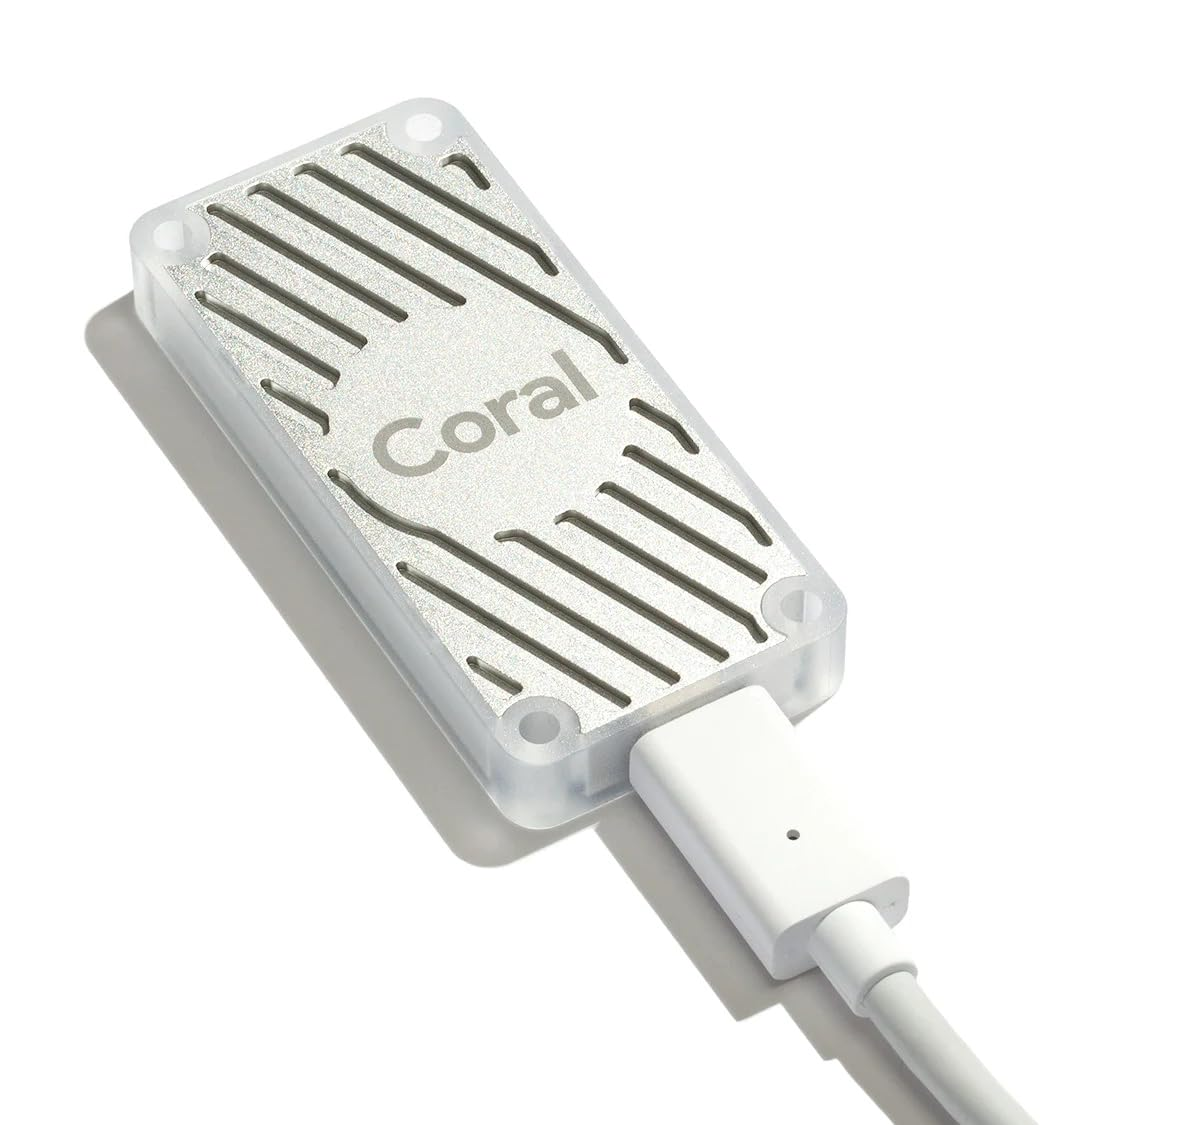
\includegraphics[width=\linewidth]{bench/img/tpu_usb.jpg}\\[3pt]
{\scriptsize Coral USB Accelerator}
\end{center}
\end{minipage}\hfill
\begin{minipage}{0.54\textwidth}
\begin{center}
\setlength{\tabcolsep}{5pt}
\renewcommand{\arraystretch}{1.15}
{\scriptsize
\begin{tabular}{ll}
\toprule
INT8 throughput  & 4 TOPS \\
Power            & $\approx$ 2 W \\
Efficiency       & 2 TOPS/W \\
On-chip memory   & 8 MB \\
Off-chip memory  & none, host only \\
Arithmetic       & INT8 only \\
Workload         & inference only \\
Host interface   & USB 3.0 \\
\bottomrule
\end{tabular}}
\end{center}
\end{minipage}

\vspace{0.5cm}

\begin{center}
{\small A systolic accelerator sized for a few watts, with no memory of its own
beyond the 8\,MB.}
\end{center}

\end{frame}
